\chapter{SYSTEM ANALYSIS}

\section{Existing System}

The existing approach to managing panchayat-level elections is predominantly manual. Voter registration is conducted at designated offices where applicants physically fill and submit forms. These forms are reviewed by local officers and added to physical voter rolls. During elections, voters present their Voter ID cards at polling booths to receive paper ballots, which are cast in physical ballot boxes and subsequently counted by hand.

The key limitations of the existing manual system include:

\begin{itemize}
    \item \textbf{No Centralised Database:} Voter records exist as physical documents with no digital backup, making retrieval and verification difficult.
    \item \textbf{Prone to Impersonation:} Without biometric or photographic verification at the time of voting, identity fraud is difficult to detect.
    \item \textbf{Slow Result Computation:} Manual ballot counting is time-consuming and susceptible to counting errors.
    \item \textbf{No Real-Time Monitoring:} Election officials have no live view of voter turnout or candidate standing during the election.
    \item \textbf{Poor Accessibility:} Voters must physically travel to offices and polling booths to participate in the electoral process.
    \item \textbf{Limited Audit Trail:} Paper records do not provide a tamper-evident audit trail, making post-election verification difficult.
\end{itemize}

\section{Proposed System}

The VoteDesk system proposes a comprehensive digital alternative that automates and secures the entire panchayat election process. The proposed system provides:

\begin{itemize}
    \item \textbf{Online Voter Registration:} Voters can register from anywhere using a web browser, with their details validated against panchayat records.
    \item \textbf{Two-Step Verification:} Email OTP verification upon registration, followed by BLO approval before voting rights are granted.
    \item \textbf{Role-Based Portals:} Dedicated dashboards for Admin, BLO, Voter, and Candidate roles with tailored functionality.
    \item \textbf{Secure Digital Voting:} Voters cast votes through an authenticated session, with live photo capture as verification.
    \item \textbf{Anonymous Vote Records:} Votes are stored without reference to the voter's identity, preserving ballot secrecy.
    \item \textbf{Real-Time Statistics:} Administrators and candidates can monitor live turnout and election progress.
    \item \textbf{Digital Result Publication:} BLOs can publish results electronically, making them immediately accessible to the public.
\end{itemize}

\section{Data Flow Analysis}

\subsection{DFD Level 0 -- Context Diagram}

\begin{figure}[H]
\centering
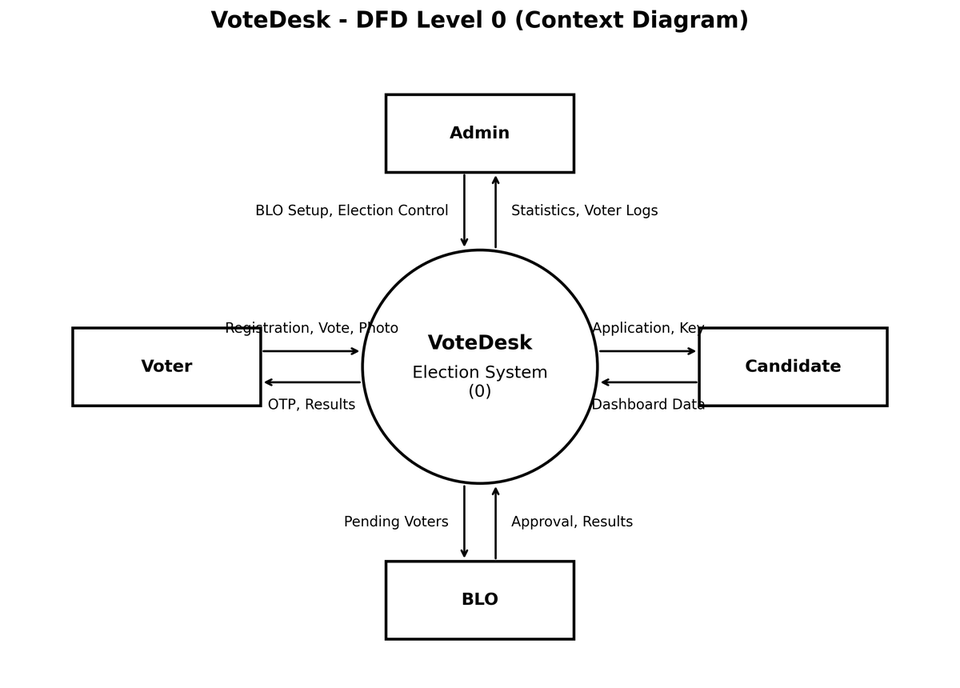
\includegraphics[width=\textwidth,height=0.75\textheight,keepaspectratio]{dfd_level0.png}
\caption{VoteDesk DFD Level 0 -- Context Diagram}
\label{fig:dfd0}
\end{figure}

The diagram represents the high-level data flow between the central election system and its primary external entities.

\subsection{DFD Level 1}

\begin{figure}[H]
\centering
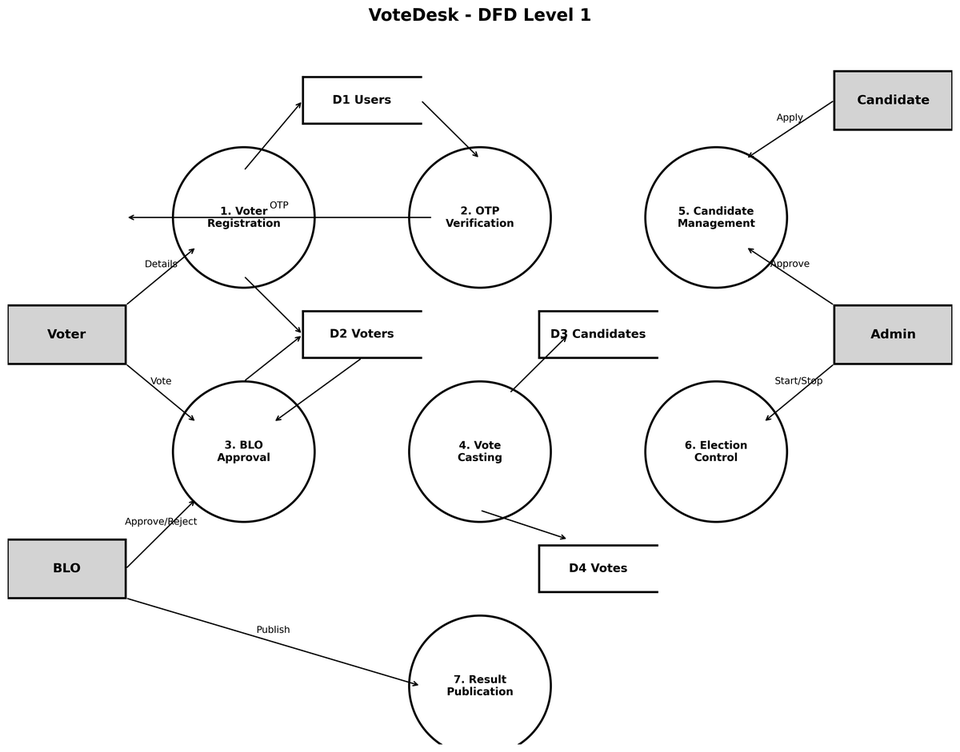
\includegraphics[width=\textwidth,height=0.75\textheight,keepaspectratio]{dfd_level1.png}
\caption{VoteDesk DFD Level 1 Diagram}
\label{fig:dfd1}
\end{figure}

The Level 1 DFD illustrates the internal sub-processes and data stores involved in the election management workflows.

\section{Functional Requirements}

\subsection{Administrator}
\begin{itemize}
    \item The system shall allow the administrator to create and manage BLO accounts with panchayat assignments.
    \item The system shall allow the administrator to activate and deactivate the election cycle.
    \item The system shall allow the administrator to approve or reject candidate applications.
    \item The system shall allow the administrator to view voter verification logs grouped by panchayat.
    \item The system shall allow the administrator to bulk delete all voters within a specific panchayat.
\end{itemize}

\subsection{Block Level Officer (BLO)}
\begin{itemize}
    \item The system shall allow BLOs to view pending voter registrations within their assigned panchayat.
    \item The system shall allow BLOs to approve or reject individual voter applications.
    \item The system shall allow BLOs to publish election results after the election ends.
    \item The system shall prevent BLOs from publishing results while the election is still active.
\end{itemize}

\subsection{Voter}
\begin{itemize}
    \item The system shall provide a registration form accepting name, date of birth, Voter ID, Aadhaar number, mobile number, email, and panchayat selection.
    \item The system shall enforce a minimum age of 18 years for voter registration.
    \item The system shall send a 6-digit OTP to the registered email address for verification.
    \item The system shall allow approved voters to log in using their email or Voter ID and password.
    \item The system shall display only candidates from the voter's registered panchayat.
    \item The system shall capture a photograph at the time of vote submission.
    \item The system shall prevent any voter from voting more than once.
\end{itemize}

\subsection{Candidate}
\begin{itemize}
    \item The system shall provide a public candidate application form.
    \item The system shall enforce a minimum age of 21 years for candidate registration.
    \item The system shall send a unique Candidate Key via email upon admin approval.
    \item The system shall allow approved candidates to log in using email, password, and Candidate Key.
    \item The system shall display voter turnout, opponent details, and approved voter lists on the candidate dashboard.
\end{itemize}

\section{Non-Functional Requirements}

\begin{itemize}
    \item \textbf{Security:} All passwords are stored using bcrypt hashing. OTPs are hashed before database storage. CSRF tokens protect all state-changing form submissions.
    \item \textbf{Performance:} Database queries use Eloquent eager loading to minimise N+1 query problems. The queue system handles email dispatch asynchronously.
    \item \textbf{Scalability:} The modular MVC architecture allows new panchayats, roles, or modules to be added without restructuring the core system.
    \item \textbf{Availability:} The application is designed for local deployment with PHP's built-in development server, and is compatible with Apache and Nginx for production.
    \item \textbf{Usability:} The system provides clear error messages, success notifications, and role-specific dashboards to ensure ease of use for non-technical end users.
    \item \textbf{Data Integrity:} Database transactions are used during vote casting to ensure that vote creation, voter status update, and candidate vote count increment are atomic operations.
    \item \textbf{Maintainability:} Code follows Laravel conventions including PSR-4 autoloading, MVC separation, and Eloquent ORM for clean database interaction.
\end{itemize}

\section{Feasibility Analysis}

\subsection{Technical Feasibility}

The system is built using Laravel 12 and PHP 8.2, which are widely supported, well-documented, and industry-standard technologies. MySQL 8.0 provides a reliable relational database backend. The Vite build tool with Tailwind CSS ensures a responsive and modern frontend. All selected technologies are open-source and freely available, reducing technical barriers.

\subsection{Economic Feasibility}

The entire technology stack is open-source and requires no licensing costs. The development environment runs on standard hardware. Hosting costs are minimal as the application can be deployed on a shared or VPS server. The elimination of paper-based processes in real-world deployment would offer significant cost savings over time.

\subsection{Operational Feasibility}

The web-based nature of the application ensures that all stakeholders can access the system using any modern web browser without requiring additional software installation. The user interface is simple and task-driven, making it accessible to users with limited technical expertise.

\section{System Environment}

\subsection{Software Environment}

\textbf{Operating System:} Windows 10/11 or Linux \\
\textbf{Backend Framework:} Laravel 12 \\
\textbf{Programming Language:} PHP 8.2+ \\
\textbf{Frontend:} Blade Templates, Bootstrap 5, Tailwind CSS 4 \\
\textbf{Build Tool:} Vite 7 \\
\textbf{Database:} MySQL 8.0+ \\
\textbf{Web Server:} PHP Built-in Server / Apache / Nginx \\
\textbf{Mail Service:} Gmail SMTP (via Laravel Mail) \\
\textbf{Development Tools:} Visual Studio Code, Composer, Git \\

\subsection{Hardware Environment}

\textbf{Processor:} Intel Core i5 or equivalent \\
\textbf{Memory (RAM):} 8 GB minimum \\
\textbf{Storage:} 256 GB SSD \\
\textbf{Operating System:} Windows 11 \\
